\documentclass{article}
\usepackage{hyperref}
\usepackage{graphicx}
\usepackage{parskip}  % http://ctan.org/pkg/parskip
\usepackage[T1]{fontenc}

% Make links look pretty in PDFs
\hypersetup{colorlinks=true, urlcolor=blue} 

\begin{document}
\title{HestiaPi Owners Manual}
\author{HestiaPi Community}
\maketitle


\section{Software}
\subsection{Quick Installation}
To make it easier for new users, HestiaPi offers ready-to-burn image files for your SD card.

If you bought your HestiaPi with an SD card, skip this step.


\subsubsection{Prepare a new SD card}

With the image file downloaded, you need to use an image writing tool (we prefer Etcher from below links) to install it on your SD card. You can't simply copy-paste it. If you downloaded a ZIP version, unzip the .img file first before the next step.

Choose the right guide for your system below (courtesy of Raspberry Pi website  thanks):

\begin{itemize}
\item \href{http://www.raspberrypi.org/documentation/installation/installing-images/linux.md}{Linux}
\item \href{http://www.raspberrypi.org/documentation/installation/installing-images/mac.md}{Mac OS}
\item \href{http://www.raspberrypi.org/documentation/installation/installing-images/windows.md}{Windows} (avoid if you can as people have reported issues flashing their card from Windows)
\end{itemize}



\subsection{Manual Installation}
For people who want to install everything step-by-step from their terminal we include all commands here. To be added...



\section{Hardware}
\subsection{PCB Soldering}
\subsubsection{Instructions}
This guide describes the steps required to solder and assemble HestiaPi Touch ONE
from parts.  Assembly with the case and wall is not covered here.

\subsubsection{Video}
\href{https://www.youtube.com/watch?v=gRcRINqT31g}{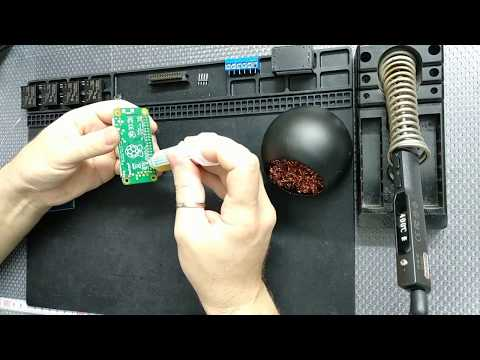
\includegraphics[width=5.0in]{img/hestiapi_one_soldering.jpg}}

\subsubsection{Hints and Tips}
The LCD needs to be connected before powering HestiaPi as it initialises on
boot only (otherwise it looks blank-white and touch events do not register) and
it may also cause a freeze or reboot due to power spike.

If you cannot control mains, that is having it off during all the time of
installation, our advise is to leave the SD card and LCD out, connect all
wires, partly (not fully) insert the SD and finish off case installation with
the LCD attached to the cover.

Once all is done, from outside of the case, push first the SD all the way in
(it does not lock-click in place) and then insert a non-metallic tool and press
the reset button from the right side. HestiaPi will boot and in about 10-15sec
the LCD will show some of the boot messages.


\subsection{Printing the Case}
Printing the case really depends on your own printer but here are some basic
guidelines that you can adjust accordingly. The power supply for HVAC - US is
too high but because we use the same design for both US and EU models, you
would need to clip off one of the 3 LCD hooks. Facing the cover from the
outside, cut the bottom left hook. Doesn't need to be flush.

\subsubsection{Files}
\href{https://hestiapi.com/downloads/}{Download} the latest (set of 2) .STL
files (BaseONE*.stl and CoverONE*.stl).

\subsubsection{Filament}
Choose a filament that stays rigid enough in the max temperature your house may
reach on a hot Summer day without the AC on :)

We use nGen filament for this reason but also because it prints easily and
reliably.  Check the same \href{https://hestiapi.com/downloads/}{download} page
for printing instructions and tips.


\subsection{Wall Installation ONE}
HestiaPi's case comes in 2 parts. The backplate that goes to the wall and
should not be visible and the front cover. The backplate should have 4 small
holes, 3 larger holes and an opening for the wires coming from the wall.

If you bought HestiaPi, all internal screws are replaced with plastic rivets.
Otherwise you would need:

\begin{itemize}
\item 4 x 2.5Mx25mm hex screws
\item 4 x 2.5M hex nuts
\end{itemize}

For attaching to the wall you need:
\begin{itemize}
\item 4 x 3.5Mx40mm non-countersunk screws
\end{itemize}

Place the hex screws through the 4 small holes entering from the side facing
the wall. Secure them in the hex slot and make sure they are sit flush. Remove
the LCD from the PCB and insert the PCB alone guiding the 4 screws through the
4 corner holes of the Pi and secure with the nuts. Avoid using a large tool.
You can simply tighten them by hand. Don't overtighten.

With the remaining 3 larger holes mark your wall and drill according to the
location of the wires. The opening of the backplate should match the location
of the wires. Secure the backplate and PCB with the 3 larger screws.

Complete wiring according to your model instructions (for US see \ref{fig:us};
for EU see \ref{fig:eu})

\begin{figure}
  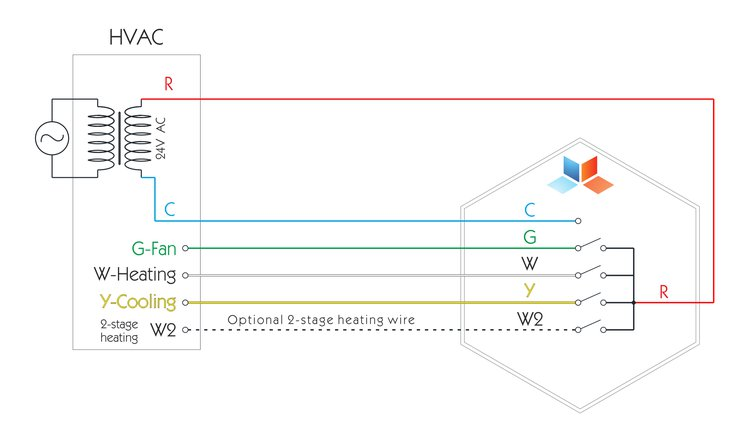
\includegraphics[width=5.0in]{img/US-hvac-wiring-diagram.jpg}
  \caption{US Wiring Diagram}
  \label{fig:us}
\end{figure}

\begin{figure}
  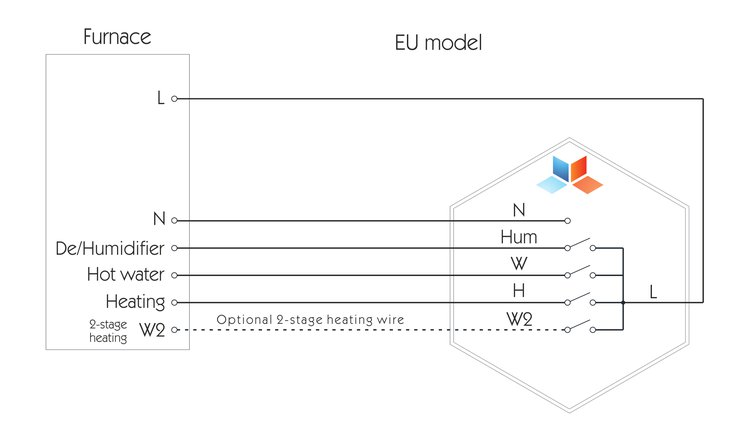
\includegraphics[width=5.0in]{img/eu-wiring-diagram.jpg}
  \caption{EU Wiring Diagram}
  \label{fig:eu}
\end{figure}

Remove any protective film from the LCD if present and lock the LCD on the
cover from the inside making sure the LCD's header is at the top.

Guide the 4 wires through the slit of bottom partition of the cover and secure
the sensor in it so that it is thermally protected from the rest of the
circuit.

If you installed the bottom screw it may block the cover to fully insert. Clip
off part of the sensor partition to allow enough clearance.

Hold the front cover aligned to the backplate and bring closer while you make
sure the pin header of the PCB is aligned to the header of the LCD. Push firmly
from the sides of the cover and not from the LCD till it locks in place. Make
sure no wires are caught in between as this may block the cover from locking in
place securely.



\section{Configuration}
\subsection{First boot}
Fix your HestiaPi's case to the wall first. If you simply want to test-drive
HestiaPi before committing to it, connect the LCD first and then plug in a
Micro USB cable to the Pi's port.

\begin{enumerate}
\item Insert the MicroSD card back in the Raspberry Pi. Just push it in. It
      does not click. It does not lock in place. A tiny part of it will stick
      out just enough to grab and pull it if needed.
\item Insert the LCD in the cover. Remove the protective film if present. Turn
      and push it in place. It should feel firm in place.
\item Take all necessary precautions before applying mains voltage so cut off
      the power now!
\item Connect all Heating, Cooling, Fan and Hot Water (depending on model)
      control lines on the terminal block's contacts.
\item Connect remaining wires, marked C(N) and R(L).
\item Place the sensor at the bottom compartment of the cover and fit the 4
      wires in the vertical slit. Note that the sensor, the little shiny
      square, should be placed facing outwards and ideally not be blocked by
      any plastic piece of the case. The red wire (Vin) goes to the top pin
      (Vin) on the PCB.
\item Align and push evenly the cover against the base aligning at the same
      times the pins with the LCD connector. The cover should lock when pushed
      all the way in. Step back and enjoy the new looks of your wall :)
\item If you cannot cut off the power on the cables, you are risking of
      HestiaPi booting before the LCD is connected. In such a scenario the LCD
      will not display anything but a blank white screen and you would need to
      restart as it is not ``plug and play'' like HDMI. We would advise to leave
      the SD card out before applying mains voltage and just before you are
      about to close the case, insert it but don't restart. It shouldn't boot.
      Once you close the case, there is a chance that it will restart. Close
      the case and wait 20 seconds. If nothing shows up on the screen, it
      didn't restart.  Press reset button from the right side.
\item If at any time you want to remove the top cover, select ``Shutdown'' from
      the App. When HestiaPi Touch is completely shut down, simply pull the
      cover outwards.
\item You should soon see the HestiaPi boot sequence and the loading screen at
      the end with a countdown. Follow
      \href{https://github.com/HestiaPi/hestia-touch-openhab/wiki/Connect-WiFi}
      {these steps} to connect your new HestiaPi to your WiFi.
\item After a few seconds the screen will show if the WiFi is connected and
      what is the local IP it got (DHCP)
\item The full installation may take up to 20 minutes for the very first time
      and a few restarts are normal. Just leave it alone. You can always SSH to
      it.  Use pi/hestia
\item The SD card image expands automatically to occupy the complete size of
      the card if available.
\item While waiting, head over to the \href{https://hestiapi.com/downloads/}{downloads}
      section and download the smartphone app on your phone. Under settings set
      Local OpenHAB URL as http://[hestiapi\_IP]:8080 and close the application
\item The LCD UI starts with 0 values or blank fields. This is normal until it
      gets ready.
\item Once the LCD is showing the UI with temperature values, try and load the
      app again or simply use your laptop and navigate to:\\
      http://[hestiapi\_IP]:8080/start/index and select ``Basic UI''
\item You should now be able to control the basic functions from either the App
      or your browser
\item Please note that the UI of the app, web and LCD may change with software
      updates so back up your customisations before running an update.
\item OpenHAB2 has a great \href{https://community.openhab.org/}{forum} with so
      much information from fellow users. Salivate at what you want to make now
      with it.
\item Feel free to explore the files under /etc/openhab2 names default.* in
      folders items, rules, sitemaps and things.
\end{enumerate}


\subsection{Boot Sequence}
To be added...


\subsection{Connect WiFi}
Follow the on-screen instructions on the LCD when it prompts to connect your
phone to the ``HESTIAPI'' network with HESTIAPI as the password. Once connected
you will automatically be prompted on your phone to select your WiFi network
from a list (no hidden SSID supported yet) and enter the password.

Your HestiaPi will then restart to connect to your network and the HESTIAPI
network will not be shown again if you entered the correct the details.



\subsection{Change Settings}
\subsubsection{Easy Remote Access}
All latest releases of HestiaPi offer very easy remote access to your home
without touching your network modem/router or even knowing HestiaPi's IP! Does
not depend on port forwarding or DynDNS! Woohooo!

\textbf{Please note that this is an externally hosted service not controlled by
you or us but by OpenHAB itself.}

\href{https://www.youtube.com/watch?v=joz5f4ejJVc}{Instructions video} (if you
prefer video to text)

To activate it (shipped disabled by default for obvious reasons) go to
http://[YOUR-HESTIAPI-IP]:8080/paperui and select Add-ons > MISC and make
sure ``openHAB Cloud Connector'' is installed.

Once installed SSH into your HestiaPi (username: pi and password: hestia) and
type:

\texttt{    cat /var/lib/openhab2/uuid}

 copy the output somewhere. Then type:

\texttt{        cat /var/lib/openhab2/openhabcloud/secret}

copy this output too. Reboot your HestiaPi

\texttt{        sudo reboot}

    
Then go to \url{https://myopenhab.org} and create an account using your details
and the above information (UUID and secret).

You can now access your HestiaPi Touch from a browser or your mobile app

Hint: Enter \url{https://myopenhab.org} as a remote url and your myopenHAB
account username and password as credentials

\subsubsection{Update Your DynDNS Automatically}
\href{https://github.com/HestiaPi/hestia-touch-openhab/blob/ONE/home/pi/scripts/getpublicip.sh}
{getpublicip.sh} does just that.

Stored with instructions here:

\texttt{    /home/pi/scripts/getpublicip.sh}

You would need an account depending on the service you choose to use inside the script.


\subsection{File Structure \& Paths}
\textbf{WiFi details}

\texttt{/etc/wpa\_supplicant/wpa\_supplicant.conf}

\textbf{OpenHAB}
Items

\texttt{/etc/openhab2/items/default.items}

Rules

\texttt{/etc/openhab2/rules/default.rules}

Sitemaps

\texttt{/etc/openhab2/sitemaps/default.sitemap}

Things

\texttt{/etc/openhab2/things/default.things}

Logs

\texttt{/var/log/openhab2/events.log\\
/var/log/openhab2/openhab.log}

\textbf{LCD UI}
The LCD UI is an HTML-based page loaded on a fullscreen browser. All HTML, CSS, JS, fonts and icon files are in here

\texttt{/home/pi/scripts/oneui}

The vue framework is used.
    
\textbf{Scripts}
In 
\texttt{/home/pi/scripts}

There are
\texttt{AdafruitDHTHum.py\\
AdafruitDHTTemp.py}

Read sensor data from DHT sensors.

\texttt{C2F.sh\\
F2C.sh}

Change HestiaPi from Celcius to Fahrenheit and vice versa.

\texttt{getBMEhumi.sh\\
getBMEtemp.sh\\
getBMEpress.sh}

Read sensor data from BME sensors (calling bme280.py).

\texttt{getcputemperature.sh}

Returns RasPi CPU temperature.

\texttt{getssid.sh}

Returns WiFi SSID name.

\texttt{gettz.sh}

Returns system Timezone.

\texttt{getuseddiskspace.sh}

Returns used SD card space.

\texttt{getwifiinfo.sh }

Returns WiFi signal strength.

\texttt{getwlan0ip.sh }

Returns WiFi IP.

\texttt{getwlan0mac.sh }

Returns WiFi MAC address.

\texttt{netcheck.sh }

Cron script that checks WiFi connectivity by pinging its gateway. If no
response is received at the first time, the WiFi interface is restarted and a
DHCP (dynamic) IP is requested. If no response is received again RaspberryPi,
the reboot command is sent. Please note this script is not enabled by default
and you will need to follow the instructions supplied at the top of the file.
Please also note that restarting the Pi will stop any current task and will not
resume after restart.

\texttt{openhabloader.sh }

Loads the Touch LCD UI.

\texttt{getpublicip.sh }

Checks current public IP and if it matches with previous reading, it does
nothing else. If current public IP is different, the latest value is sent to
your account (manual and free account registration needed).
    
\textbf{Web UI}

\texttt{http://[YOUR\_HESTIA\_IP]:8080/basicui/app}

or simply


\texttt{http://[YOUR\_HESTIA\_IP]:8080}

and then select Basic UI and default

\textbf{Smartphone App}
Under Settings > Local server settings


\texttt{http://[YOUR\_HESTIA\_IP]:8080}



\section{FAQ}
\subsection{Configuration}
\subsubsection{Default SSH Username and Password}

Username: pi

Password: hestia

SSH port: 22

\subsubsection{MQTT Configuration}
All the topics are defined in the .things
\href{https://github.com/HestiaPi/hestia-touch-openhab/wiki/File-Structure-&-Paths-ONE}{file}.

Confirm by subscribing from another laptop to all (\#) MQTT IDs and listen for
published messages while you play with your HestiaPi. For Linux users, run this
in a terminal:

\texttt{mosquitto\_sub -h [HESTIA\_PI\_IP] -d -t hestia/\#}

\subsubsection{How to Access My HestiaPi From Outside My House}

You will need a WiFi router with port forwarding feature (most routers do these
days) and if you don’t have a static IP (or if you don’t know what this is),
you will need to use a free Dynamic DNS service called
\href{https://www.noip.com/support/knowledgebase/install-ip-duc-onto-raspberry-pi/}{NoIP}.
Don’t worry -- although we can’t offer support on individual routers, we can
certainly point you in the right direction. Installation instructions on the
above link.  Alternatively you can use my.openhab.org which is a service hosted
externally and is not controlled by us or you but by OpenHAB itself. Go to:

\texttt{http://[YOUR-HESTIAPI-IP]:8080/paperui}

and select Add-ons > MISC and install ``openHAB Cloud Connector'' if not
installed. Once installed SSH into your HestiaPi (username: pi and password:
hestia) and type:

\texttt{cat /var/lib/openhab2/uuid}

write the output down. Then type:

\texttt{cat /var/lib/openhab2/openhabcloud/secret}

write this output down too.

Then go to \url{https://myopenhab.org} and create an account using your details
and the above information (UUID and secret). You can now access your HestiaPi
Touch from a browser or your mobile app (enter ``\url{https://myopenhab.org}''
as a remote url and your myopenHAB account username and password as
credentials).  The above steps are also available in youtube format
\href{https://www.youtube.com/watch?v=joz5f4ejJVc}{here} too.


\subsection{Troubleshooting}
\subsubsection{How to edit files via SSH}
If you are very new to command line interface we would advise you taking a
short online course by searching for ``linux command line interface'' on your
favourite website.

To edit a file while you are inside SSH use the command

\texttt{sudo nano /path/to/your/file}

Then leave your mouse alone as it does not control you cursor anymore

Use only your keyboard and once you are done, press Ctrl+O to save and Ctrl+X to close.

\subsubsection{Start OpenHAB2 in Debug Mode}

For OpenHAB2 (v10.x image -- July 2018)
To monitor the OpenHAB logs without stopping the service run

\texttt{openhab-cli showlogs}

To start OpenHAB manually after stopping the service run

\texttt{openhab-cli start}

For older OpenHAB installations:
Stop OpenHAB first

\texttt{sudo service openhab2 stop}

and when it is stopped, start it manually

\texttt{/usr/share/openhab2/start\_debug.sh}

once (if) loaded type inside the OpenHAB session

\texttt{log:tail}

and notice any issues.


\end{document}

